\section{Motivations}
\label{sec:motivations}
\blue{Section~\ref{sec:mot_stability} shows that phase tokens are stable and low-dimensional, and Section~\ref{sec:mot_changes} identifies the changes across cycles that this stability does not cover.}
%Real-world sequences are inherently non-stationary, often exhibiting distributional shifts in their cyclical patterns. Recent forecasting models increasingly adopt patch-based representations, where sequences are segmented into cycles—either known or estimated—and each cycle is treated as a fundamental modeling unit. This inductive bias supports a variety of architectures, from patch-based Transformers that align tokens with seasonal XXXXXs (e.g., PatchTST) to models that explicitly encode seasonal components (e.g., TimeBase). However, these approaches implicitly assume distributional invariance across patches, effectively treating seasonal segments as temporally stable. In practice, non-stationarity induces cycle drifts through time-varying amplitudes or subtle frequency modulations. Such shifts distort the intra-patch distribution and undermine robustness when patches are the sole modeling unit.

%To address this limitation, we adopt a complementary phase-centric perspective, treating intra-patch positions as tokens, a strategy we term \emph{phase tokenization}.Intuitively, the impact of cycle drift on phase tokens is confined to only a subset of phases. Even within this subset, the effect manifests primarily as a uniform amplitude shift, which is comparatively easier to accommodate. Moreover, phase-based averaging across patches tends to be more robust to local perturbations. These observations motivate the exploration of phase tokenization.

\begin{figure*}[t]
  \centering
  %  subfigure
  \begin{subfigure}[t]{0.59\textwidth}
    \centering
    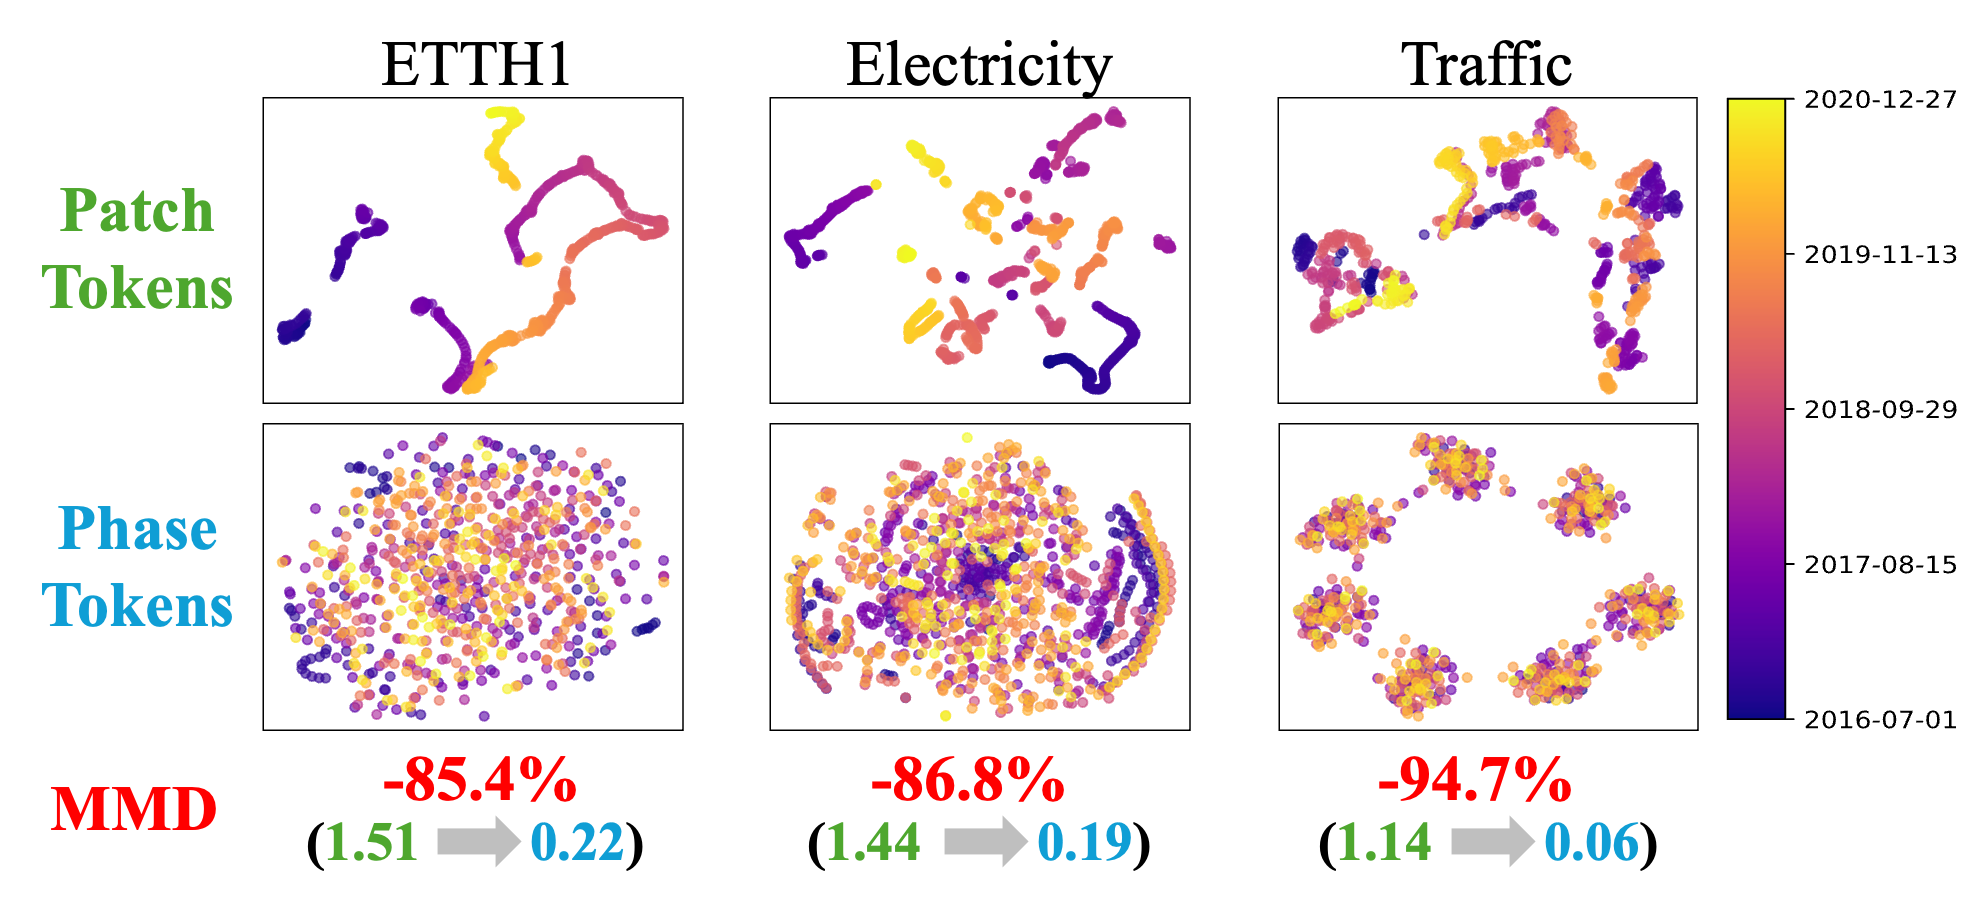
\includegraphics[width=\linewidth]{figures/visualization_cycle_phase_comparison.png}
    \caption{Temporal shift comparison across multiple datasets.}
    \label{fig:visualization_tsne}
  \end{subfigure}
  \hfill
%  subfigure
  \begin{subfigure}[t]{0.37\textwidth}
    \centering
    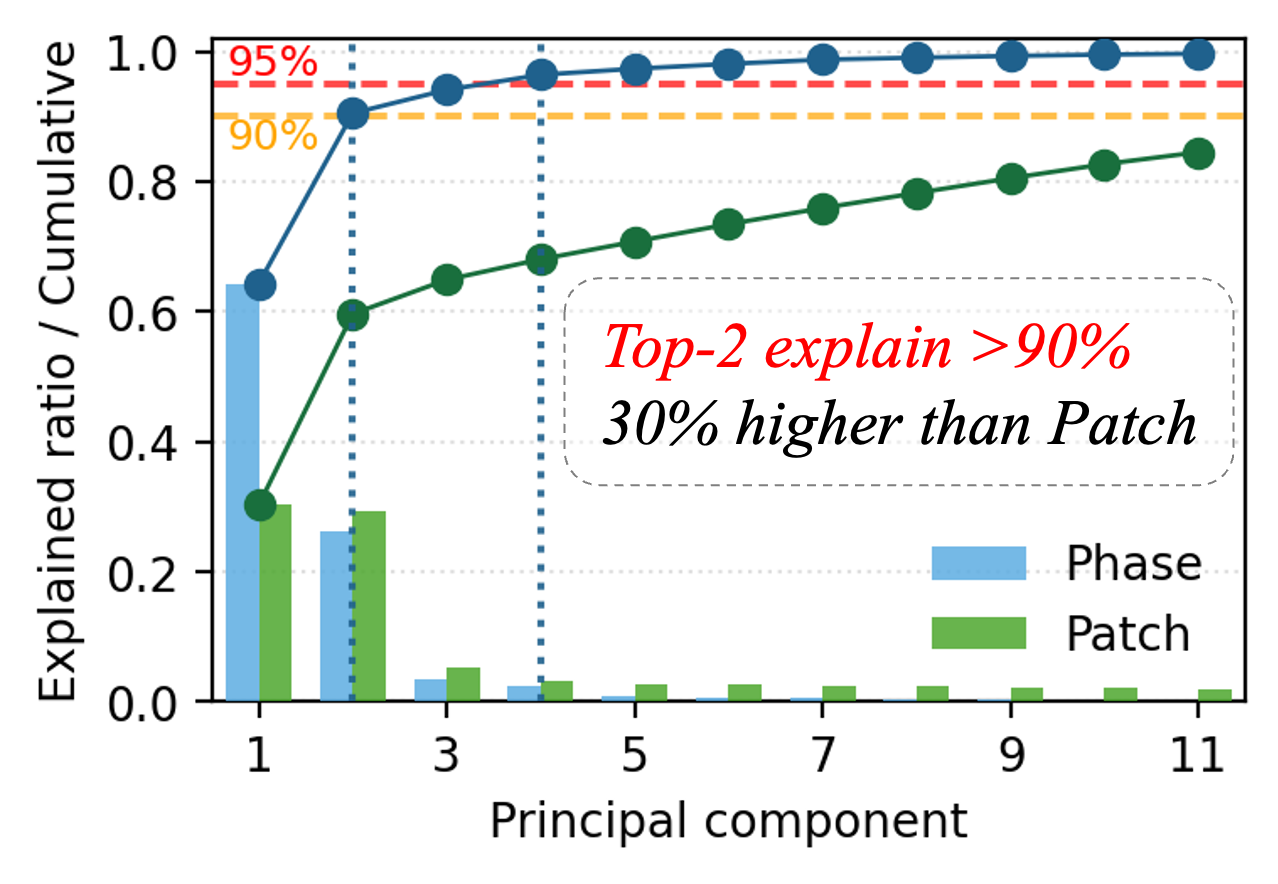
\includegraphics[width=\linewidth]{figures/traffic_pca_cycle_phase.png}
    \caption{PCA for phase tokens on \emph{Traffic}.}
    \label{fig:traffic_pca_cycle_phase}
  \end{subfigure}
  \caption{Visualization of phase tokenization and its advantages.  
  (a) Phase tokenization yields more stable representations than patch-based embeddings.
  (b) Phase tokens exhibit clear low-dimensionality compared with patch tokens.}  
  \label{fig:phase_token_comparison}
\end{figure*}


\subsection{\blue{Phase Tokens Are Stable and Low-Dimensional}}
\label{sec:mot_stability}

To motivate our approach, we conduct a comparative analysis of the geometric structures of patch and phase tokens across three widely used datasets. 
As illustrated in \figref{fig:phase_token}, a patch token is composed of adjacent observations within a local period, whereas a phase token is constructed by extracting values at identical offsets across consecutive periods. We gain the following two important insights from the thorough analysis. 


\fakeparagraph{Insight 1: Phase tokens are globally stationary, while patch tokens are locally stationary}
To provide an intuitive overview of their geometric structures, we project both types of tokens into two-dimensional spaces using t-SNE~\citep{tsne2008}.
As shown in Fig.~\ref{fig:visualization_tsne}, the distributions of patch tokens drift continuously over time but exhibit local coherence, indicating \emph{local stationarity} and supporting the minimal impact of excluding cycle patterns from intensive processing. In contrast, phase tokens form compact and coherent clusters that remain stable over the long term, reflecting strong \emph{global stationarity}. To rigorously quantify the long-term drift, we compute the average discrepancy distance between each subsequent week and the initial week. Specifically, we adopt the Maximum Mean Discrepancy (MMD) metric~\citep{ouyang2021mmd}, a statistical measure of distributional divergence:
\begin{equation}
\begin{aligned}
\mathrm{MMD}^2(P, Q)
&= \mathbb{E}_{x,x' \sim P}[k(x,x')]
+ \mathbb{E}_{y,y' \sim Q}[k(y,y')]\\
&\quad - 2\,\mathbb{E}_{x \sim P, y \sim Q}[k(x,y)],
\end{aligned}
\end{equation}
where \(P\) and \(Q\) denote tokens collected from two different weeks, respectively, and \(k(\cdot,\cdot)\) is the RBF kernel function. As two distributions become closer, their MMD value approaches zero. The results at the bottom of Fig.~\ref{fig:visualization_tsne} show that the average MMD distance of the phase token space is significantly smaller than that of the patch token space. Taken together, both qualitative and quantitative analyses demonstrate that phase tokenization exhibits substantially lower temporal distribution divergence, thereby \emph{facilitating better generalization across the time axis}.

\fakeparagraph{Insight 2: Phase tokens reside in a lower-dimensional subspace than patch tokens}
To measure the effective dimensionality of the token space, we perform principal component analysis (PCA) on it. Surprisingly, as illustrated in Fig.~\ref{fig:traffic_pca_cycle_phase}, two dimensions are already sufficient to explain over 90\% of the variance of phase tokens, whereas patch tokens require more than eleven dimensions to achieve the same degree of explanation, owing to their drifting behavior observed in Fig.~\ref{fig:visualization_tsne}. Consequently, phase information resides in a low-dimensional subspace, \emph{providing a principled basis for parameter- and computation-efficient modeling}.

\revised{
We further establish, using perturbation theory, that phase tokenization remains stable under perturbations of cycle patterns, whereas patch tokenization exhibits structural drift. 
To formalize this result, we represent a univariate periodic sequence as a two-dimensional matrix via delay embedding and analyze the structural properties of this embedded matrix.
}
Due to space limitations, only the core theorem is presented here, while the detailed proof is provided in \blue{the electronic supplement}.
\begin{theorem}[Phase Tokenization Stability]
\label{thm:stability}
Let $X = A G^\top + N \in \mathbb{R}^{D\times H}$ with 
$\operatorname{rank}(A)=\operatorname{rank}(G)=r \ll \min(D,H)$, 
and consider the transformed data
\begin{equation}
X' = X S^\top + R,
\end{equation}
where \blue{$M=AG^\top$ is the signal and $N'=NS^\top$ the transformed noise, so that} $\|N'\|_2 \le \|S\|_2\|N\|_2$, 
$\|R\|_2 \le \varepsilon(\|M\|_F+\|N\|_F)$, 
and let $\delta_{\min} > 0$ denote the minimal spectral separation. 
Then there exists a universal constant $C>0$ such that:
\begin{enumerate}[leftmargin=2em]
\item For phase tokenization and corresponding subspace $\mathcal U_r$, there exists:
\begin{equation}
d\big(\mathcal U_r(X),\mathcal U_r(X')\big)
\;\le\;
C\,\frac{\|N\|_2+\|N'\|_2+\|R\|_2}{\delta_{\min}},
\end{equation}
with exact invariance in the noiseless case $(N=R=0)$.
\item For patch tokenization and corresponding subspace $\mathcal V_r$, there exists:
\begin{equation}
\begin{aligned}
d\big(\mathcal V_r(X),\mathcal V_r(X')\big)
\;\ge\;&
d\big(\mathrm{Col}(G),\mathrm{Col}(S G)\big)\\
&- C\,\frac{\|N\|_2+\|N'\|_2+\|R\|_2}{\delta_{\min}}.
\end{aligned}
\end{equation}
\end{enumerate}
\end{theorem}

\noindent
\textbf{Takeaways.} 
Phase tokenization is structurally invariant under the cycle pattern change $S$ and only subject to perturbations from noise and small day-to-day mismatches. 
In contrast, patch tokenization generally suffers from a non-vanishing structural offset. 
Hence, \emph{phase tokenization is more robust and consistent under cycle pattern drifts}.


\blue{
\subsection{Changes Across Cycles}
\label{sec:mot_changes}

\begin{figure}[t]
\centering
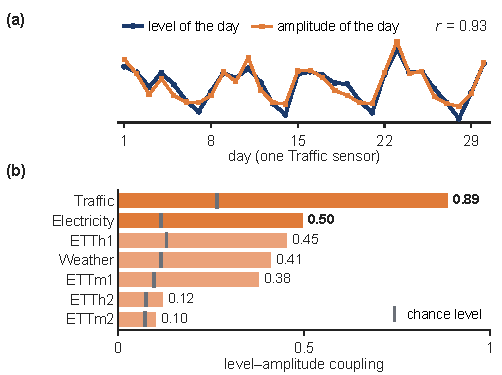
\includegraphics[width=\linewidth]{figures/coupling.pdf}
\caption{Level--amplitude coupling: busier days swing wider. (a)~Thirty days of one Traffic sensor from the test period, a window whose correlation (0.93) is close to the Traffic median; top: hourly occupancy; bottom: the level (mean) and the amplitude (RMS deviation) of each day, standardized. (b)~Sign-consistent coupling over the test windows of every dataset; red ticks: the shifted-pairing reference. A cycle has 24 samples, one day on the hourly datasets.}
\label{fig:coupling}
\end{figure}

\fakeparagraph{What Theorem~\ref{thm:stability} does not cover}
The theorem covers a \emph{common shape change}: $X'=XS^\top$ reshapes every cycle of a window in the same way. Sensor streams also change from one cycle to the next (Fig.~\ref{fig:coupling}(a)). The \emph{level} of a cycle, its mean, moves: a road carries more traffic on some days than on others. The \emph{amplitude} of a cycle, its swing around the level, moves with the level: on a busy day the rush hours rise far above the night, whereas a quiet day stays low and flat. In the folded matrix $X\in\mathbb R^{D\times H}$ of the theorem, with the $D$ cycles as rows and the $H$ phases as columns, these two \emph{changes across cycles} take the form
\begin{equation}
\underbrace{X+\ell\,\mathbf 1^\top}_{\text{level drift}},
\qquad
\underbrace{\operatorname{diag}(\mathbf 1+\alpha\ell)\,X}_{\text{level-dependent amplitude}},
\label{eq:cycle_axis_changes}
\end{equation}
where $\ell\in\mathbb R^D$ holds the cycle levels and $\alpha$ is a coupling strength. Unlike $XS^\top$, which mixes the columns, both act on the rows, so in general neither leaves the span of the phase tokens, $\operatorname{Col}(X)$, unchanged, and Theorem~\ref{thm:stability} no longer applies. With noise, the two changes combine into
\begin{equation}
X_{kp}=\ell_k+(1+\alpha\ell_k)\,s_p+e_{kp},
\qquad
\ell_k=\ell_{k-1}+\eta_k,
\label{eq:mult_model}
\end{equation}
where $X_{kp}$ is the value at phase $p$ of cycle $k$, with a zero-mean seasonal profile $s$, a random-walk level $\ell$ and Gaussian noise. With $\alpha=0$ this is the additive seasonal random-walk model; with $\alpha\neq0$ the swing grows with the level, and we call it the multiplicative seasonal model, after the multiplicative form of Holt--Winters forecasting~\citep{winters1960forecasting}. Under \equref{eq:mult_model}, the phase token of phase $p$ is $s_p\mathbf 1+(1+\alpha s_p)\,\ell$ up to noise: every phase token carries the level, but with a weight that follows the cycle shape, large at the rush hours and small at night. Level-dependent amplitude thus moves the phase tokens specifically, since it multiplies each row, that is, each patch token, by one factor and leaves the span of the patch tokens unchanged.

\fakeparagraph{Insight 3: The within-cycle amplitude moves with the cycle level}
We measure the amplitude of a cycle as its root-mean-square deviation from its mean. In Fig.~\ref{fig:coupling}(a), the levels and amplitudes of the 30 days rise and fall together, with a correlation of 0.93. We compute this correlation for every channel and every window of 720 samples (30 cycles of 24, stride 24), directly on the data. Over 30 cycles, two series that drift independently also correlate by chance, with either sign. We therefore average the correlation over the windows of each channel, keeping its sign, and report the mean magnitude of these channel averages, the \emph{sign-consistent coupling}: chance correlations cancel in the average, a coupling of stable sign does not. As a reference, the same statistic is computed after pairing the levels of every window with the amplitudes of the window half the period away, which keeps the drift of both but removes their alignment.

Fig.~\ref{fig:coupling}(b) shows that five benchmarks lie far above this reference and that the coupling is strongest on the two sensor networks: Electricity, with 321 meters, reaches 0.50, and Traffic, with 862 road sensors, 0.89. On these two networks the correlation is positive in 84\% and in over 99\% of the windows, respectively, so a busier day swings wider. Weekends do not explain this: over the weekday cycles of each window alone, the coupling is still 0.51 and 0.82. On ETTh1 and ETTm1, the sign differs between channels but is stable within each, so the amplitude grows with the level on some channels and shrinks on others. ETTh2 and ETTm2 show the weakest coupling, little above the reference. On the training and validation periods, too, the two sensor networks are the most and ETTh2 and ETTm2 the least coupled (electronic supplement). Hence, \emph{wherever its sign is stable, a phase-token model must produce a cycle shape that scales with the level}.

This coupling within a window does not contradict Insight~1, which compares the distribution of phase tokens across weeks. Section~\ref{sec:extension} adds one component to \sysname for each of the two changes, and Section~\ref{sec:theory} shows why each takes its form and that the coupling forces an error floor only where it drives the amplitude beyond an envelope that the trained weights fix, which Section~\ref{sec:exp_envelopes} measures.
}
